\documentclass[12pt]{article}

\usepackage{times}
\usepackage{textcomp}
\usepackage{listings}
\usepackage{fullpage}
\usepackage{color}
\usepackage{hyperref} 
\usepackage{pst-tree} 
\usepackage{verbatim} 
\usepackage{graphicx}
\usepackage{amsmath,amsfonts,amssymb,amsthm}
\graphicspath{ {./}} 

\def\part#1{\item[\bf #1)]}
\renewcommand{\thesubsection}{Question \arabic{subsection}}

\author{Clement Tsang}

\begin{document}

\begin{center}
\Large\textbf{CS 241, Lecture 10 - Context Free Grammars, Parse Trees, and Parsing}
\end{center}
\begin{center}
\textbf{Thurs, Feb 07, 2019}
\end{center}

\section{CFGs}
\begin{itemize}
    \item Consider the arithmetic operations over $\Sigma = \{a, b, c, +, -, *, /, (, )\}$.  Find a CFG for the following:
        \begin{itemize}
            \item $L_1$: Arithmetic expressions from $\Sigma$ without parentheses
            \item $L_2$: Well formed arithmetic expressions from $\Sigma$ with balanced parentheses
        \end{itemize}
        Also, find a derivation for $a - b$ in the first language and for $(a - b)$ in the second one.
    \item Solutions: \\
        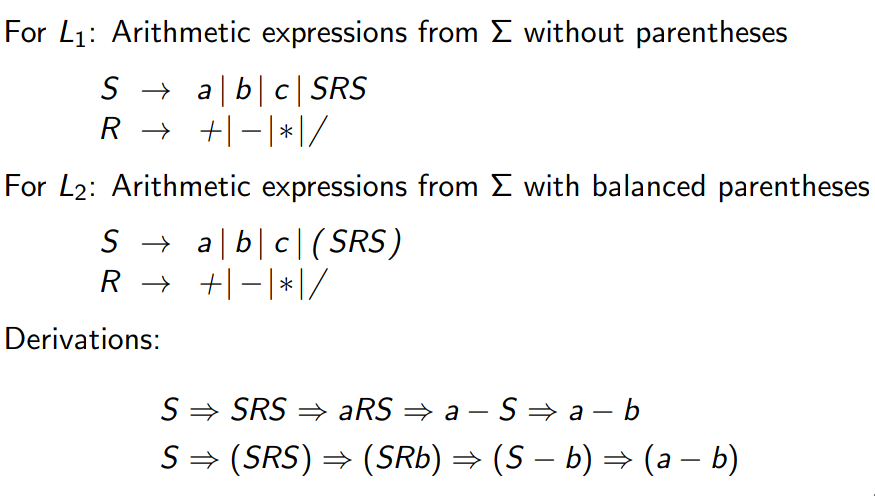
\includegraphics[scale=0.4]{cfg_example.png}
    \item Using the above language, let us create a \textbf{parse tree} for the input of $a-b$:\\
        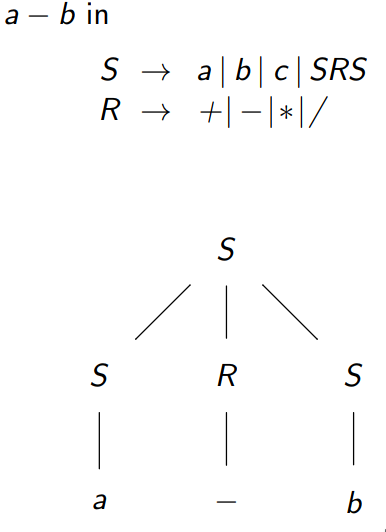
\includegraphics[scale=0.4]{parse_tree_one.png}
    \item Another example: using $aaabbb$ in $S \rightarrow \epsilon | aSb$ :\\
        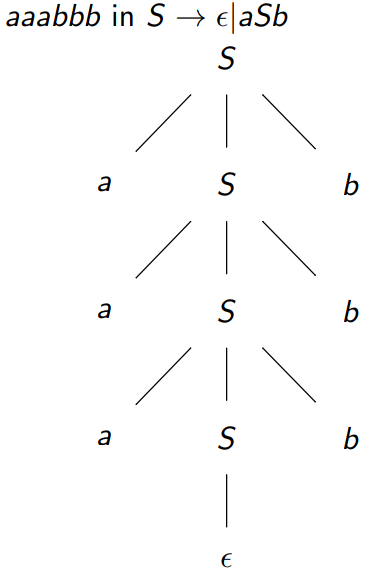
\includegraphics[scale=0.4]{parse_tree_two.png}
    \item We note that for every left/right-most derivation, there exists a unique parse tree, and vice versa.
    \item We also note that given a grammar, every left/right derivation for a string is NOT unique.  For example, consider two left-most $a - b * c$: \\
        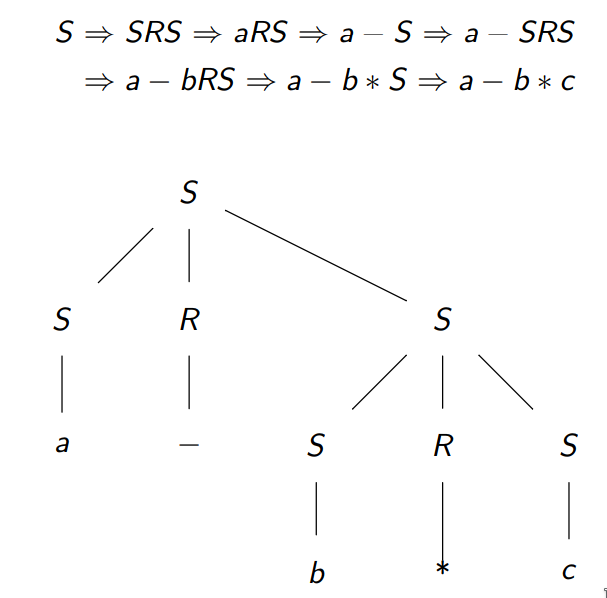
\includegraphics[scale=0.4]{parse_tree_three.png} \\
        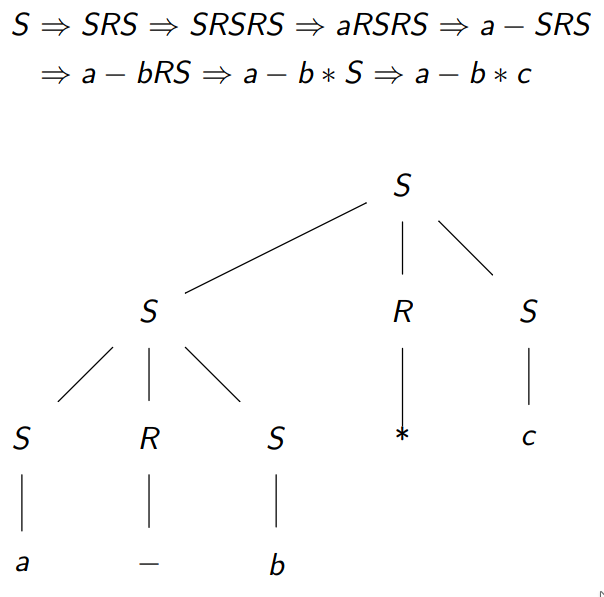
\includegraphics[scale=0.5]{parse_tree_four.png}
    \item We define a grammar for which some word has more than one distinct leftmost/rightmost derivation/parse tree is called an \textbf{ambiguous grammar}.  Our example above is an ambiguous example.
    \item So how can we remove ambiguity?  Well, we covered this in rustcc - create \emph{precedence} to force your parse tree to understand, say, $a - b * c$ as $a - (b * c)$, NOT $(a - b) * c$!
    \item This make it unambiguous.  This is what $L_2$ does in our earlier example.
    \item What we can also do is insist on what associativity we are using (ie: force right associatve grammar for $a - b * c$.
    \item If $L$ is a context-free language, is there always an unambiguous grammar s.t. $L(G) = L$?  No!  
    \item Can we write a computer program to recognize whether a grammar is ambiguous or not?  No!
    \item This means that given two CFGs $G_1$ and $G_2$, we cannot determine if $L(G_1) == L(G_2)$ or even something easier like $L(G_1) \hat L(G_2) = \varnothing$.  They are both undecideable problems.
    \item What we \emph{can} do is use pushdown automation, which are just machines that are basically DFAs with an additional stack that we can process in LIFO order.  
    \item But we also need to find the \textbf{derivation} - finding this derivation is called \textbf{parsing}.
\end{itemize}

\section{Parsing}
\begin{itemize}
    \item Top-down Parsing:
        \begin{itemize}
            \item Start with $S$ and store intermediate derivations in a stack, and match characters to $w$.
            \item Then every time we pop from the stack, we will have that consumed input $+$ reverse of stack is equal to a intermediate step in our derivation - that is, a step is an $\alpha_i$ where $S \Rightarrow \dots \Rightarrow \alpha_i \Rightarrow \dots \Rightarrow w$.
            \item We will augment our grammar to include $\vdash$ and $\dashv$ symbolizing the beginning and end of the file.  We also include a new start state, $S'$, to begin our parsing.
            \item Our original CFG $G = (N, \Sigma, P, S)$ becomes
                \begin{align*}
                G = (N \cup \{S'\}, \Sigma \cup \{\vdash, \dashv\}, P \cup \{S' \rightarrow \vdash S \dashv\}, S')
                \end{align*}
            \item The algorithm can be coded as follows: \\
                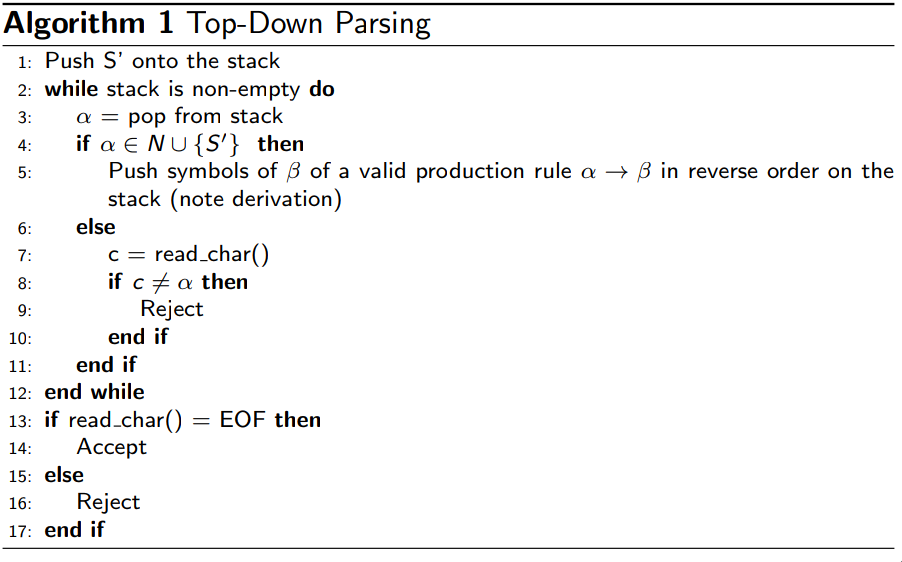
\includegraphics[scale=0.4]{tdparse.png}
        \end{itemize}
        \newpage
    \item Example: Let us determine whether or not $w = abcdef$ is inside $L(G)$ where 
        $$G = (\{S, A, B\}, \{a, b, c, d, e, f\}, P, S)$$ 
        is defined with P given by:
        \begin{align*}
            S &\rightarrow AcB \\
            A &\rightarrow ab\\
            A &\rightarrow ff\\
            B &\rightarrow def\\
            B &\rightarrow ef 
        \end{align*}
    \item Solution: We first augment the grammar with $S' \rightarrow \vdash S \dashv$, and look for $w = \vdash abcdef \dashv$ in this augmented grammar: \\
        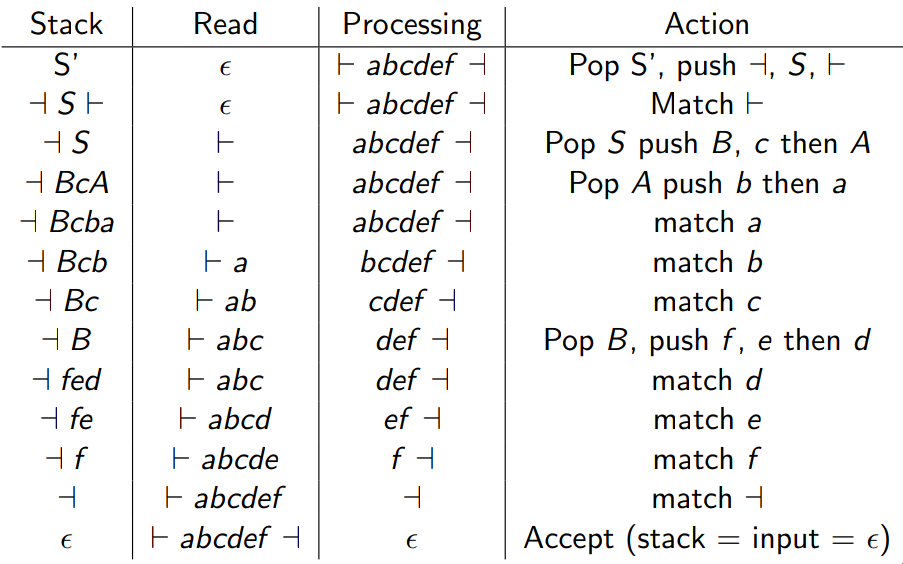
\includegraphics[scale=0.4]{parsing.png}
\end{itemize}

\section{Correction}
\begin{itemize}
    \item Determining if $L(G) = \not0$ is decideable.
\end{itemize}

\end{document}

